\section{Traditional sampling methods}
\label{chap:sm}
\subsection{Inverse transform sampling}
\label{sec:sm:inverse_transform}

In the one-dimensional case, this amounts to converting a uniform random variable (which are easy to generate) into a variable sampled from a general distribution \(f(\theta)\). One first finds its cumulative distribution function (CDF):
\begin{equation}
  F(\theta) = \int\limits_{-\infty}^\theta f(\theta^\prime) \d{\theta^\prime},
\end{equation}
computes the inverse of the CDF, and then applies this function to a uniform random variable  \(x\sim U(0,1)\) to generate a variable \(\theta = F^{-1}(x)\), which is distributed according to \(f(\theta)\). 

In the general \(D\)-dimensional case, one calculates \(D\) conditional distributions \(\{f_i:i=1\ldots,D\}\): by marginalising over parameters with indices greater than \(i\) and conditioning on parameters with indices less than \(i\):
%
\begin{equation}
  f_i(\theta_i|\theta_{i-1},\ldots,\theta_1) 
  =
  \frac{%
    \int f_i(\params) d\theta_{i+1}\ldots \d{\theta_{N}}
  }{%
    \int f_i(\params) d\theta_{i}\ldots \d{\theta_{N}}
  },
\end{equation}
%
Integrating these yields \(D\) conditional CDFs:
%
\begin{equation}
  x_i = F_i(\theta_i|\theta_{i-1},\ldots,\theta_1) = \int\limits_0^{\theta_i} f_i(\theta_i^\prime|\theta_{i-1},\ldots,\theta_1) \d{\theta_i^\prime}.
\end{equation}
%
Inverting this gives \(\theta_i = F^{-1}_i(x_i|\theta_{i-1},\ldots,\theta_1)\), which constitutes a set of relations sequentially transforming \(D\) uniform random variables \(\{x_i\}\) into \(\{\theta_i\}\) distributed according to \(f(\params)\).

In many cases, the prior \(\prior(\params)\) is separable, and the above equations are easily calculated. For sections of the parameters which are not separable, the calculation can become more involved. We include a few demonstrations of this procedure in Section~\ref{sec:pc:prior_transformations}. In the language of nested sampling the \(D\) uniform random variables \(x_i\) are termed elements of the ``unit hypercube'' and \(\theta_i\) are elements of the ``physical space''.

\subsection{Prior transformations}
\label{sec:pc:prior_transformations}
Here we give examples of the procedure for calculating the transformation from the unit hypercube to the physical space. We demonstrate it for a separable case, and a more complicated dependent case

To recap, we aim to compute the inverse of the functions \(F_i\): 
\begin{equation}
  F_i(\theta_i|\theta_{i-1},\ldots,\theta_0) = \int\limits_0^{\theta_i} \pi_i(\theta_i^\prime|\theta_{i-1},\ldots,\theta_1) d\theta_i^\prime,
  \label{eqn:pc:appFi}
\end{equation}
%
where:
%
\begin{equation}
  \pi_i(\theta_i|\theta_{i-1},\ldots,\theta_0) 
  =
  \frac{%
    \int \pi_i(\params) d\theta_{i+1}\ldots d\theta_{N}
  }{%
    \int \pi_i(\params) d\theta_{i}\ldots d\theta_{N}
  }.
  \label{eqn:pc:apppii}
\end{equation}
\(\bFF\) maps from \(\params\) in the physical space onto the unit hypercube injectively. 



\subsubsection{Separable priors}
\label{sec:pc:separable_priors}
A separable prior satisfies:
\begin{equation}
  \pi(\params) = \prod_i\pi_i(\theta_i).
  \label{eqn:pc:separability}
\end{equation}
This has the fortunate side effect that the functions \(F_i\) only depend on \(\theta_i\):
\begin{equation}
  F_i(\theta_i|\theta_{i-1},\ldots,\theta_0) = F_i(\theta_i).
\end{equation}

Solving a separable prior thus amounts to solving a one-dimensional inverse-transform sampling problem. We demonstrate this procedure for two cases, a rectangular uniform prior, and a Gaussian prior.

\subsubsection{Uniform prior}
\label{sec:pc:uniform_prior}
%------------ commands for this section --------------
\newcommand{\thetamin}{\theta_\smin} % Minimum uniform prior
\newcommand{\thetamax}{\theta_\smax} % Maximum uniform prior
%-----------------------------------------------------
A rectangular uniform prior is defined by two parameters, \({\thetamin,\thetamax}\):
\begin{equation}
  \pi(\theta) = 
  \left\{
    \begin{array}{rl}
      {(\thetamax - \thetamin)}^{-1} 
      &
      \text{for }\thetamax<\theta_i<\thetamin \\
      0 & \text{otherwise.}
    \end{array}
  \right.
\label{eqn:pc:uniform_prior}
\end{equation}

Computing \(F(\theta)\) we find:
\begin{align}
  F(\theta) &= \int_{-\infty}^\theta \pi(\theta')d\theta', \nonumber\\
  &= \frac{\theta-\thetamin}{\thetamax-\thetamin},
  \label{eqn:pc:calc_uniform_trans}
\end{align}
with \(F=0\) or \(1\) either side of \(\thetamin\) and \(\thetamax\) respectively. Inverting the equation \(F(\theta)=x\) we find:
\begin{equation}
  \theta = \thetamin+(\thetamax-\thetamin)x,
  \label{eqn:pc:uniform_trans}                           
\end{equation}
is the transformation from \(x\) in the unit hypercube to \(\theta\) in the physical space.

\subsubsection{Gaussian prior}
\label{sec:pc:gaussian_prior}
Defining a Gaussian prior with mean \(\mu\) and standard deviation \(\sigma\):
\begin{equation}
  \pi(\theta) = \frac{1}{\sqrt{2\pi}\sigma}\exp{\left[-\frac{{(x-\mu)}^2}{2\sigma^2}\right]},
  \label{eqn:pc:gaussian_prior}
\end{equation}
We find that the procedure above yields:
\begin{equation}
  \theta = \mu + \sqrt{2}\sigma\text{erfinv}(2x-1),
  \label{eqn:pc:gaussian_trans}                           
\end{equation}
where \(\text{erfinv}\) is the conventional inverse error function.




\subsubsection{Forced identifiability priors}
\label{sec:pc:forced_identifiablility}

As an example of a prior that is not separable in the parameters, we consider a forced identifiability prior. Here, \(n\) parameters are distributed uniformly between \(\thetamin\) and \(\thetamax\), but subject to the constraint that they are ordered numerically. This is a particularly useful prior in the reconstruction of functions using a spline with movable knots~\citep{vazquez_knots,knottedsky1,knottedsky2,planck2015-a24}. In this case, the  horizontal locations of the knots must be ordered.

The required prior is uniform in the hyper-triangle defined by \(\thetamin<\theta_1<\cdots<\theta_n<\thetamax\), and zero everywhere else:
%
\begin{equation}
  \pi(\params) = 
  \left\{
    \begin{array}{rl}
      \frac{1}{n!{(\thetamax - \thetamin)}^{n}} 
      &
      \text{for }\thetamin<\theta_1<\cdots<\theta_n<\thetamax \\
      0 &\text{otherwise.}
    \end{array}
    \right.
\label{eqn:pc:sorted_uniform_prior}
\end{equation}

To calculate equations~\eqref{eqn:pc:appFi} \&~\ref{eqn:pc:apppii} we integrate over the constant distribution, taking care with the limits. We find:
\begin{align}
  \pi_i(\theta_i|\theta_{i-1},\ldots,\theta_0) &= \frac{(n-i+1){(\theta_i-\theta_{i-1})}^{n-i}}{{(\thetamax-\thetamin)}^{n-i+1}},\\
  F_i(\theta_i|\theta_{i-1},\ldots,\theta_0) &= {\left(\frac{\theta_i-\theta_{i-1}}{\thetamax-\theta_{i-1}}\right)}^{n-i+1},
  \label{eqn:pc:sorted_uniform_calc}
\end{align}
where for consistency we define \(\theta_0 = \thetamin\). Hence solving \(x_i=F(\theta_i|\theta_{i-1},\ldots,\theta_0)\) for \(\theta_i\) we find:
\begin{equation}
  \theta_i = \theta_{i-1}+ (\thetamax-\theta_{i-1})x_i^{1/(n-i+1)}.
  \label{eqn:pc:sorted_uniform_trans}
\end{equation}
This enables \(\{\theta_i\}\) to be calculated sequentially from \(\{x_i\}\). We may interpret this transformation as \(\theta_i\) being distributed as the smallest of \(n-i+1\) uniformly distributed variables in the range \([\theta_{i-1},\thetamax]\).



\subsection{Rejection sampling}
\label{sec:sm:rejection}

The principle behind rejection sampling is simple, and best demonstrated graphically as in Figure~\ref{fig:sm:rej}. If one requires some samples from a complicated distribution \(f(x)\), but has the knowledge that it satisfies \(f(x)<g(x)\) for some simpler distribution \(g(x)\), then one may sample from \(g\), and accept only those samples with probability less than \(f\). 

\begin{figure}[tp]
  \tikzsetnextfilename{rejection}
  \centering
  \includegraphics[width=\textwidth]{appendices/sampling_methods/plots/rejection.tikz}
  \caption{Rejection sampling. One may produce samples from some complicated distribution \(f(x)\) using a simpler distribution \(g(x)\) provided that \(g(x)>f(x)\) within the domain of interest. One samples from \(g\), and accepts only those samples that lie under the \(f\) curve.\label{fig:sm:rej}}
\end{figure}

Obviously this will be very inefficient unless \(g(x)\) happens to be rather close to \(f(x)\). One finds that in general this inefficiency is exaggerated by the curse of dimensionality.

\subsection{Metropolis---Hastings}
\label{sec:sm:mh}
Metropolis---Hastings approaches are an extremely widely used methodology for generating a sequence of samples (or points) from some posterior \(\posterior(x)\).

A sequence of \(T\) points is termed a {\em chain\/} \(\chain_T\):
\begin{equation}
  \chain_T = \{ x^{(t)}: t=1\cdots T \}.
\end{equation}
A new point \(x^{(t+1)}\) is generated from a proposal density \(\proposal\) which depends on the current state \(x^{(t)}\). Typically \(\proposal(x|x^{(t)})\) might be a Gaussian distribution centered on the current value of \(x^{(t)}\):
\begin{equation}
  \log \proposal(x|x^{(t)}) = \text{const} -\frac{{\left[ x-x^{(t)} \right]}^2}{2\varepsilon^2},
\end{equation}
but in general the proposal density can be any fixed density from which we may draw samples easily.

A new state \(x\) is proposed from the proposal density \(\proposal(x|x^{(t)})\), and it is accepted with probability:
\begin{equation}
  p_\mathrm{accept}(x|x^{(t)}) = \frac{\posterior(x)}{\posterior(x^{(t)})}\frac{\proposal(x^{(t)}|x)}{\proposal(x|x^{(t)})}.
\end{equation}
If the step is accepted, then \(x^{(t+1)}=x\), otherwise \(x^{(t+1)} = x^{(t)}\). This procedure can be seen schematically in Figure~\ref{fig:sm:MH}.
\begin{figure}[tp]
  \centering
  \tikzsetnextfilename{MH}
  \includegraphics[width=\textwidth]{appendices/sampling_methods/plots/MH.tikz}
  \caption{Metropolis-Hastings. Here we have some degenerate two-dimensional posterior \(\posterior\), and a circular proposal distribution \(\proposal\).\label{fig:sm:MH}}.
\end{figure}


This has the distinct advantage that it does not require one to take into account the overall normalisation of the posterior, circumnavigating any issues associated with computing the evidence \(\ev\), since:
\begin{equation}
  \frac{\posterior(x)}{\posterior(x^{(t)})} \equiv
  \frac{\lik(x)\prior(x)}{\lik(x^{(t)})\prior(x^{(t)})}.
\end{equation}
It is important to note that the chain \(C_T\) will comprise \(T\) samples which are {\em correlated}. If the proposal distribution amounts to a random walk with step size \(\varepsilon<\sigma_{\min{}}\), and the longest lengthscale in the probably region is \(\sigma_{\max{}}\)  then one will expect: \(\tau \sim {(L/\varepsilon)}^2\). If \(\varepsilon>\sigma_{\min{}}\), then one starts to expect a very low acceptance rate, so typically for a isotropic random walk, the timescale on which one expects to generate independent samples is:
\begin{equation}
  \tau \sim \left( \frac{\sigma_{\max{}}}{\sigma_{\min{}}} \right).
\end{equation}
In theory, given that the above relation has no dimensionality attached to it, Metropolis Hastings can be extremely successful in high dimensions. However, there are several issues.

First, one does not initially a-priori have a good starting point. There is therefore a period of ``burn-in'' attached to MH methods. Knowing when this period is truely over, and one is starting to generate random samples can be challenging in the general case.

In many cases, \(\tau\gg1\) resulting in unacceptable run-times. This can be ameliorated by choosing a proposal distribution \(\proposal\) that better agrees with the posterior \(\posterior\). However, this amounts to adding in many effective tuning parameters. Many algorithms work by having a ``learning'' phase, whereby the algorithm deduces for itself a good correlated Gaussian proposal distribution, but given the fact that this is not strictly Markovian care must be taken.



\subsection{Slice sampling}
\label{sec:sm:slice}
Radford Neal initially proposed slice sampling as an effective methodology for generating samples numerically from a given posterior \(\posterior(\params)\). One first chooses a `slice' (or probability level) \(\posterior_0\) uniformly within \([0,\posterior_\smax]\). One then samples uniformly within the \(\params\)-region defined by \(\posterior(\params)>\posterior_0\). The similarity with the iso-likelihood contour sampling required by nested sampling should be clear. In the one-dimensional case, he suggests the sampling procedure detailed in Figure~\ref{fig:bay:1d_slice}.

\begin{figure}[tp]
  \centerline{%
    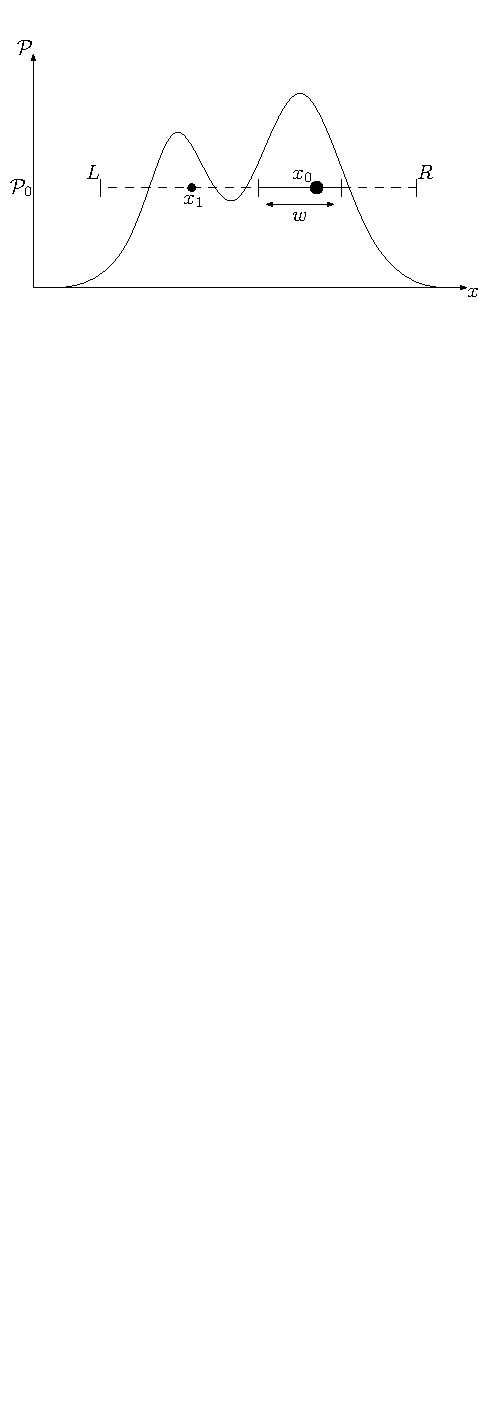
\includegraphics[width=\textwidth]{appendices/sampling_methods/figures/slice}
  }

  \caption{Slice sampling in one dimension. 
    Given a probability level (or slice) \(\posterior_0\), slice sampling samples within the horizontal region defined by \(\posterior>\posterior_0\). 
    From an initial point \(x_0\) within the slice (\(\posterior(x_0)>\posterior_0\)), a new point \(x_1\) is generated within the slice with a distribution \(P(x_1|x_0)\).
    External bounds are first set on the slice \(\hat{L}<x_0<\hat{R}\) by uniformly expanding a random initial bound of width \(w\) until they lie outside the slice (Neal terms this the {\em stepping out\/} procedure). 
    \(x_1\) is then sampled uniformly within these bounds.  
    If \(x_1\) is not in the slice, then \(\hat{L}\) or \(\hat{R}\) is replaced with \(x_1\), ensuring that \(x_0\) is still within the slice.
    This procedure is guaranteed to generate a new point \(x_1\), and satisfies detailed balance \(P(x_0|x_1) = P(x_1|x_0)\). Thus, if \(x_0\) is drawn from a uniform distribution within the slice, so is \(x_1\).\label{fig:bay:1d_slice}
  }
\end{figure}



In higher dimensions,~\cite{NealSlice} suggests a variety of MCMC-like methods. The simplest of these is implemented by sampling each of the parameter directions in turn. Since each one-dimensional slice requires \(\bigO{\text{a few}}\) likelihood calculations, the number of likelihood calculations required scales linearly with dimensionality, providing the region is efficiently navigated. Multi-dimensional slice sampling has many of the benefits of a traditional MH approach, and uses a proposal distribution which is much more efficient at sampling a hard likelihood constraint.

\subsection{Thermodynamic integration}
The traditional method of computing the evidence from MCMC procedures is via {\em thermodynamic integration}.
The aim is to compute:
\begin{equation}
  \ev = \int \lik(\Theta) \prior(\Theta) \d{\Theta}.
\end{equation}
Inspired by thermodynamics, we define the posterior \(\posterior_\beta \propto \lik^\beta\prior\) at temperature \(\beta\) as:
\begin{align}
  \posterior_\beta(\Theta) &= \frac{\lik^{\beta}(\Theta) \prior(\Theta)}{\ev_\beta}, 
  \label{eqn:bay:posteriorb}
  \\
  \ev_\beta &= \int\lik^{\beta}(\Theta) \prior(\Theta) \d{\Theta}.
  \label{eqn:bay:evb}
\end{align}
If the likelihood is interpreted as a Boltzmann-like probability distribution, then:
\begin{equation}
{\lik(\Theta)}^\beta = \exp[-\beta E(\Theta)],
\end{equation}
is the Boltzmann probability of finding a system with inverse temperature \(\beta = T^{-1}\) in state \(\Theta\) with energy \(E\), and the partition function is \(\ev_\beta\).

Inspired by thermodynamics, one can see that:
\begin{equation}
  \frac{\d{}}{\d{\beta}}\log\ev_\beta = \frac{\int  \lik^\beta \prior \log\lik\d{\Theta}}{\int\lik\prior \d{\Theta}} = \int \posterior_\beta \log\lik\d{\Theta} =  \mean{\log\lik}_\beta.
  \label{eqn:bay:thermo}
\end{equation}
Hence, integrating the above equation yields:
\begin{equation}
  \log\ev_1-\log\ev_0 = \log\ev = \int_{0}^{1}\mean{\log\lik}_\beta.
  \label{eqn:sm:thermo}
\end{equation}
The key point is that we may compute the mean \(\mean{\log\lik}_\beta\) from a set of samples from the posterior \(\posterior_\beta\). If we therefore generate a set of samples for a range of temperatures \(\beta\), the one-dimensional integral above may be computed easily. Thermodynamic calculation of the evidence therefore is equivalent to running multiple MCMC runs at several temperatures.
This however suffers from the disadvantage that it is difficult to produce an estimate of the error in computing~\eqref{eqn:sm:thermo}. 

